\documentclass[]{article}
\usepackage{amsmath}
\usepackage{amsfonts}
\usepackage{amssymb}
\usepackage{amsthm}
\usepackage{bm}
\usepackage{cancel}
\usepackage{graphicx}
\usepackage{pdfpages}
\usepackage{hyperref}

\renewcommand{\thesection}{\arabic{section}}
\renewcommand{\thesubsection}{\thesection.\alph{subsection}}
\renewcommand{\thesubsubsection}{\thesubsection.\roman{subsubsection}}

\newtheorem{genthm}{Theorem}

\newcommand{\unit}[1]{\bm{\hat{#1}}}
\newcommand{\iprod}[2]{\left\langle #1, #2 \right\rangle}
\newcommand{\tpose}[1]{\left[#1\right]^{\! \top} \!\!}

%opening
\title{EECS 16A HW14}
\author{Bryan Ngo}
\date{2019-12-07}

\begin{document}

\maketitle

\section{How Much is Too Much?}

\subsection{}

Yes, the higher-degree polynomials are affected by noise. 
Around degree 15, the best fit polynomial starts to deviate heavily from the set. 

\subsection{}

According to the graph, it is beneficial to pick polynomial fits greater than first-order. 
However, this is clearly \emph{not} the trend that is indicated in the data set, even if a degree 15 polynomial is the most beneficial. 

\section{OMP Exercise}

\begin{equation}
	\underbrace{\begin{bmatrix}
		1 & 1 & 0 & -1 \\
		1 & 0 & -1 & 0 \\
		0 & 1 & 1 & 1
		\end{bmatrix}}_{\bm{M}}
	\underbrace{\begin{bmatrix}
		x_1 \\
		x_2 \\
		x_3 \\
		x_4
		\end{bmatrix}}_{\bm{x}} \approx 
	\underbrace{\begin{bmatrix}
		4 \\
		6 \\
		3
		\end{bmatrix}}_{\bm{b}}
\end{equation}
Finding the greatest inner product, 
\begin{center}
\begin{tabular}{c|c}
	\(i\) & \(\iprod{\bm{m}_i}{\bm{b}}\) \\
	\hline
	1 & \(10\) \\
	2 & \(7\) \\
	3 & \(-3\) \\
	4 & \(-1\)
\end{tabular}
\end{center}
we see that \(\bm{m}_1\) has the largest inner product. 
The rejection of \(\bm{b}\) onto \(\bm{m}_1\) is now
\begin{equation}
	\bm{b}' = \bm{b} - \frac{\iprod{\bm{m}_1}{\bm{b}}}{\iprod{\bm{m}_1}{\bm{m}_1}} \bm{m}_1 = \begin{bmatrix}
	4 \\
	6 \\
	3
	\end{bmatrix} - 5 \begin{bmatrix}
	1 \\
	1 \\
	0
	\end{bmatrix} = \begin{bmatrix}
	-1 \\
	1 \\
	3
	\end{bmatrix}
\end{equation}
Finding the largest inner product with \(\bm{b}'\), 
\begin{center}
\begin{tabular}{c|c}
	\(i\) & \(\iprod{\bm{m}_i}{\bm{b}'}\) \\
	\hline
	1 & \(0\) \\
	2 & \(2\) \\
	3 & \(2\) \\
	4 & \(4\)
\end{tabular}
\end{center}
Using least squares to find \(x_1, x_4\), 
\begin{align}
	\tpose{\bm{A}} \bm{A} &= \begin{bmatrix}
	1 & 1 & 0 \\
	-1 & 0 & 1
	\end{bmatrix}
	\begin{bmatrix}
	1 & -1 \\
	1 & 0 \\
	0 & 1
	\end{bmatrix} = 
	\begin{bmatrix}
	2 & -1 \\
	-1 & 2
	\end{bmatrix} \overset{\bm{A}^{-1}}{\Rightarrow} 
	\frac{1}{3} \begin{bmatrix}
	2 & 1 \\
	1 & 2
	\end{bmatrix} \\
	\tpose{\bm{A}} \bm{b} &= \begin{bmatrix}
	1 & 1 & 0 \\
	-1 & 0 & 1
	\end{bmatrix}
	\begin{bmatrix}
	4 \\
	6 \\
	3
	\end{bmatrix} = 
	\begin{bmatrix}
	10 \\
	-1
	\end{bmatrix} \\
	\unit{x} &= \frac{1}{3} \begin{bmatrix}
	2 & 1 \\
	1 & 2
	\end{bmatrix}
	\begin{bmatrix}
	10 \\
	-1
	\end{bmatrix} = 
	\begin{bmatrix}
	19 / 3 \\
	8 / 3
	\end{bmatrix} \\
	\bm{x} &= \begin{bmatrix}
	19 / 3 \\
	0 \\
	0 \\
	8 / 3
	\end{bmatrix}
\end{align}

\section{Greedy Algorithm for Calculating Matrix Eigenvalues}

\subsection{}

\begin{equation}
	\bm{Q} = \tpose{\bm{A}} \bm{A} = \begin{bmatrix}
	1 & 2 \\
	3 & 4
	\end{bmatrix}
	\begin{bmatrix}
	1 & 3 \\
	2 & 4
	\end{bmatrix} = 
	\begin{bmatrix}
	5 & 11 \\
	11 & 25
	\end{bmatrix} = \tpose{\bm{Q}}
\end{equation}

\begin{genthm}
	For some matrix \(\bm{A} \in \mathbb{R}^{2 \times 2}\), \(\bm{Q} = \tpose{\bm{A}} \bm{A}\) is symmetric. 
\end{genthm}

\begin{proof}
\begin{equation}
	\bm{Q} = \tpose{\bm{A}} \bm{A} = \begin{bmatrix}
	a_{11} & a_{12} \\
	a_{21} & a_{22}
	\end{bmatrix}
	\begin{bmatrix}
	a_{11} & a_{21} \\
	a_{12} & a_{22}
	\end{bmatrix} = 
	\begin{bmatrix}
	a_{11}^2 + a_{12}^2 & a_{11} a_{21} + a_{12} a_{22} \\
	a_{21} a_{11} + a_{22} a_{12} & a_{21}^2 + a_{22}^2
	\end{bmatrix}
\end{equation}
By inspection, it is clear that the off-diagonal entries are equal, so \(\tpose{\bm{Q}} = \bm{Q}\). 
\end{proof}

\subsection{}

\begin{genthm}
	For some matrix \(\bm{V} = \begin{bmatrix}
	\bm{v}_1 & \bm{v}_2 & \cdots & \bm{v}_N
	\end{bmatrix} \in \mathbb{R}^{N \times N}\) such that  \(\iprod{\bm{v}_i}{\bm{v}_j} = 0, i \ne j\), then \(\tpose{\bm{V}} \bm{V} = \bm{I}\). 
\end{genthm}

\begin{proof}
\begin{align}
	\tpose{\bm{V}} \bm{V} = \begin{bmatrix}
	\bm{v}_1 \\
	\bm{v}_2 \\
	\vdots \\
	\bm{v}_N
	\end{bmatrix}
	\begin{bmatrix}
	\bm{v}_1 & \bm{v}_2 & \cdots & \bm{v}_N
	\end{bmatrix} &= 
	\begin{bmatrix}
	\iprod{\bm{v}_1}{\bm{v}_1} & \iprod{\bm{v}_1}{\bm{v}_2} & \cdots & \iprod{\bm{v}_1}{\bm{v}_N} \\
	\iprod{\bm{v}_2}{\bm{v}_1} & \iprod{\bm{v}_2}{\bm{v}_2} & \cdots & \iprod{\bm{v}_2}{\bm{v}_N} \\
	\vdots & \vdots & \ddots & \vdots \\
	\iprod{\bm{v}_N}{\bm{v}_1} & \iprod{\bm{v}_N}{\bm{v}_2} & \cdots & \iprod{\bm{v}_N}{\bm{v}_N}
	\end{bmatrix} \\
	&= \begin{bmatrix}
	\|\bm{v}_1\|^2 & \iprod{\bm{v}_1}{\bm{v}_2} & \cdots & \iprod{\bm{v}_1}{\bm{v}_N} \\
	\iprod{\bm{v}_2}{\bm{v}_1} & \|\bm{v}_2\|^2 & \cdots & \iprod{\bm{v}_2}{\bm{v}_N} \\
	\vdots & \vdots & \ddots & \vdots \\
	\iprod{\bm{v}_N}{\bm{v}_1} & \iprod{\bm{v}_N}{\bm{v}_2} & \cdots & \|\bm{v}_N\|^2
	\end{bmatrix} \\
	&= \begin{bmatrix}
	1 & 0 & \cdots & 0 \\
	0 & 1 & \cdots & 0 \\
	\vdots & \vdots & \ddots & \vdots \\
	0 & 0 & \cdots & 1
	\end{bmatrix} = \bm{I}
\end{align}
\end{proof}

\subsection{}

\begin{proof}
In order to prove \(\operatorname{col}(\bm{V})\) is a basis on \(\mathbb{R}^N\), we must prove
\begin{itemize}
	\item linear independence
	\item full span of \(\mathbb{R}^N\)
\end{itemize}
If \(\operatorname{col}(\bm{V})\) were to be linearly independent, then \(\operatorname{null}(\bm{V}) = \{\bm{0}\}\). 
By definition of the nullspace, there is some vector \(\bm{x}\) such that 
\begin{align}
	\bm{V} \bm{x} &= \bm{0} \\
	\tpose{\bm{V}} \bm{V} \bm{x} &= \tpose{\bm{V}} \bm{0} \\
	\bm{I} \bm{x} &= \bm{x} = \bm{0}
\end{align}
where we use the result from \textbf{3.b}. \\
In order to prove full span of \(\mathbb{R}^N\), any vector must be represented as a linear combination of \(\operatorname{col}(\bm{V})\). 
Again, suppose some \(\bm{x}\) such that 
\begin{equation}
	\bm{V} \bm{x} = \bm{y}
\end{equation}
Since we proved earlier that \(\operatorname{col}(\bm{V})\) has linearly independent columns, \(\bm{V}\) is invertible. This means that for any \(\bm{x} \in \mathbb{R}^N\), \(\bm{x} = \bm{V}^{-1} \bm{y}\). 
\end{proof}

\subsection{}

\begin{align}
	\iprod{\bm{v}_i}{\bm{b}} &= \tpose{\bm{v}_i} (\alpha_1 \bm{v}_1 + \alpha_2 \bm{v}_2 + \cdots + \alpha_N \bm{v}_N) \\
	&= \alpha_1 \cancel{\tpose{\bm{v}_i} \bm{v}_1} + \alpha_2 \cancel{\tpose{\bm{v}_i} \bm{v}_2} + \cdots + \alpha_i \tpose{\bm{v}_i} \bm{v}_i + \cdots + \alpha_N \cancel{\tpose{\bm{v}_i} \bm{v}_N} \\
	&= \alpha_i \|\bm{v}_i\|^2 = \alpha_i
\end{align}

\subsection{}

The key here is representing \(\bm{b}\) as
\begin{equation}
	\bm{b} = \alpha_1 \bm{v}_1 + \alpha_2 \bm{v}_2 + \cdots + \alpha_N \bm{v}_N = \begin{bmatrix}
	\bm{v}_1 & \bm{v}_2 & \cdots & \bm{v}_N
	\end{bmatrix}
	\begin{bmatrix}
	\alpha_1 \\
	\alpha_2 \\
	\vdots \\
	\alpha_N
	\end{bmatrix} = \bm{V} \bm{\alpha}
\end{equation}
The least squares solution is
\begin{align}
	\tpose{\bm{V}} \bm{V} &= \bm{I} \overset{\bm{V}^{-1}}{\Rightarrow} \bm{I} \\
	\tpose{\bm{V}} \bm{b} &= \tpose{\bm{V}} \bm{V} \bm{\alpha} = \bm{I} \bm{\alpha} = \bm{\alpha} \\
	\unit{x} &= (\tpose{\bm{V}} \bm{V})^{-1} \tpose{\bm{V}} \bm{b} = \bm{I} \bm{\alpha} = \bm{\alpha} \\
	\|\bm{V}\unit{x} - \bm{b}\| &= \|\bm{V}\bm{\alpha} - \bm{b}\| = 0
\end{align}

\subsection{}

\begin{align}
	\tpose{\bm{V}_2} \bm{V}_2 &= \begin{bmatrix}
	\bm{v}_2 \\
	\vdots \\
	\bm{v}_N
	\end{bmatrix}
	\begin{bmatrix}
	\bm{v}_2 & \cdots & \bm{v}_N
	\end{bmatrix} = 
	\begin{bmatrix}
	\iprod{\bm{v}_2}{\bm{v}_2} & \cdots & \iprod{\bm{v}_2}{\bm{v}_N} \\
	\vdots & \ddots & \vdots \\
	\iprod{\bm{v}_N}{\bm{v}_2} & \cdots & \iprod{\bm{v}_N}{\bm{v}_N}
	\end{bmatrix} = \bm{I}_{N - 1} \\
	\tpose{\bm{V}_2} \bm{b} &= \begin{bmatrix}
	\bm{v}_2 \\
	\vdots \\
	\bm{v}_N
	\end{bmatrix}
	\begin{bmatrix}
	\bm{v}_1 & \bm{v}_2 & \cdots & \bm{v}_N
	\end{bmatrix}
	\bm{\alpha} = 
	\begin{bmatrix}
	\iprod{\bm{v}_2}{\bm{v}_1} & \iprod{\bm{v}_2}{\bm{v}_2} & \cdots & \iprod{\bm{v}_2}{\bm{v}_N} \\
	\vdots & \vdots & \ddots & \vdots \\
	\iprod{\bm{v}_N}{\bm{v}_1} & \iprod{\bm{v}_N}{\bm{v}_2} & \cdots & \iprod{\bm{v}_N}{\bm{v}_N} \\
	\end{bmatrix} \bm{\alpha} \\
	&= \begin{bmatrix}
	0 & 1 & 0 & \cdots & 0 \\
	0 & 0 & 1 & \cdots & 0 \\
	\vdots & \vdots & \vdots & \ddots & \vdots \\
	0 & 0 & 0 & \cdots & 1
	\end{bmatrix} \bm{\alpha} = \begin{bmatrix}
	\alpha_2 \\
	\vdots \\
	\alpha_N
	\end{bmatrix} \\
	\unit{x} &= (\tpose{\bm{V}_2} \bm{V}_2)^{-1} \tpose{\bm{V}_2} \bm{b} = \bm{I}_{N - 1} \begin{bmatrix}
	\alpha_2 \\
	\vdots \\
	\alpha_N
	\end{bmatrix} = \begin{bmatrix}
	\alpha_2 \\
	\vdots \\
	\alpha_N
	\end{bmatrix} \\
	\|\bm{V}_2\unit{x} - \bm{b}\| &= \left\|\begin{bmatrix}
	\bm{v}_2 & \cdots & \bm{v}_N
	\end{bmatrix}
	\begin{bmatrix}
	\alpha_2 \\
	\vdots \\
	\alpha_N
	\end{bmatrix} - 
	\begin{bmatrix}
	\bm{v}_1 & \bm{v}_2 & \cdots & \bm{v}_N
	\end{bmatrix}
	\begin{bmatrix}
	\alpha_1 \\
	\alpha_2 \\
	\vdots \\
	\alpha_N
	\end{bmatrix}\right\| \\
	&= \left\|(\alpha_2 \bm{v}_2 + \cdots + \alpha_N) - (\alpha_1 \bm{v}_1 + \alpha_2 \bm{v}_2 + \cdots + \alpha_N)\right\| = \|-\alpha_1 \bm{v_1}\| = \alpha_1
\end{align}

\subsection{}

Step 1 is justified since
\begin{equation}
	\tpose{\bm{V}} \bm{v}_1 = \begin{bmatrix}
	\bm{v}_1 \\
	\bm{v}_2 \\
	\vdots \\
	\bm{v}_N
	\end{bmatrix} \bm{v}_1 = 
	\begin{bmatrix}
	\iprod{\bm{v}_1}{\bm{v}_1} \\
	\iprod{\bm{v}_2}{\bm{v}_1} \\
	\vdots \\
	\iprod{\bm{v}_N}{\bm{v}_1}
	\end{bmatrix} = 
	\begin{bmatrix}
	\|\bm{v}_1\|^2 \\
	0 \\
	\vdots \\
	0
	\end{bmatrix} = 
	\begin{bmatrix}
	1 \\
	0 \\
	\vdots \\
	0
	\end{bmatrix}
\end{equation}
Step 2 is justified since 
\begin{equation}
	\begin{bmatrix}
	\lambda_1 & 0 & \cdots & 0 \\
	0 & \lambda_2 & \cdots & 0 \\
	\vdots & \vdots & \ddots & \vdots \\
	0 & 0 & \cdots & \lambda_N
	\end{bmatrix}
	\begin{bmatrix}
	1 \\
	0 \\
	\vdots \\
	0
	\end{bmatrix} = 
	\begin{bmatrix}
	\lambda_1 \\
	0 \\
	\vdots \\
	0
	\end{bmatrix}
\end{equation}
by simple matrix-vector multiplication. 
Step 3 is justified since
\begin{equation}
	\begin{bmatrix}
	\bm{v}_1 & \bm{v}_2 & \cdots & \bm{v}_N
	\end{bmatrix}
	\begin{bmatrix}
	\lambda_1 \\
	0 \\
	\vdots \\
	0
	\end{bmatrix} = 
	\lambda_1 \bm{v}_1
\end{equation}
by simple matrix-vector multiplication. 

\subsection{}

\begin{genthm}
	\(\bm{v}_1 \in \operatorname{null}(\bm{Q}_2)\) where \(\bm{Q} - \lambda_1 \bm{v}_1 \tpose{\bm{v}_1}\). 
\end{genthm}

\begin{proof}
\begin{align}
	\bm{Q}_2 \bm{v}_1 &= (\bm{Q} - \lambda_1 \bm{v}_1 \tpose{\bm{v}_1}) \bm{v}_1 \\
	&= \bm{Q} \bm{v}_1 - \lambda_1 \bm{v}_1 \tpose{\bm{v}_1} \bm{v}_1 \\
	&= \lambda_1 \bm{v}_1 - \lambda_1 \bm{v}_1 \iprod{\bm{v}_1}{\bm{v}_1} \\
	&= \lambda_1 \bm{v}_1 - \lambda_1 \bm{v}_1 = \bm{0}
\end{align}
\end{proof}

\begin{genthm}
	\(\bm{v}_2, \ldots, \bm{v}_N\) are the eigenvectors of \(\bm{Q}_2\). 
\end{genthm}

\begin{proof}
\begin{align}
	\bm{Q}_2 &= \bm{Q} - \lambda_1 \bm{v}_1 \tpose{\bm{v}_1} \\
	&= \sum_{i = 1}^{N} \lambda_i \bm{v}_i \tpose{\bm{v}_i} - \lambda_1 \bm{v}_1 \tpose{\bm{v}_1} \\
	&= \sum_{i = 2}^{N} \lambda_i \bm{v}_i \tpose{\bm{v}_i}
\end{align}
Note that this is simply the definition of \(\bm{Q}\) shifted one index up. 
This indicates that all \(\lambda_i\) for \(i \in \{2, \ldots, N\}\) are eigenvalues of \(\bm{Q}_2\). 
Using the proof in \textbf{3.g}, it is elementary to prove that \(\bm{v}_i\) are the eigenvectors associated with the eigenvalues, respectively. 
\end{proof}

\subsection{}

\begin{enumerate}
	\item Perform \(f(\bm{Q})\). Put the eigenvalue in the list. 
	\item Let \(\bm{Q} = \bm{Q} - \lambda_{max} \bm{v}_{max} \tpose{\bm{v}_{max}}\). 
	This step effectively "removes" the largest eigenvalue so far. 
	\item Repeat Step 1 until there are no eigenvalues left in \(\bm{Q}\). 
\end{enumerate}

\section{Sparse Imaging}

\subsection{}

See Jupyter Notebook. 

\subsection{}

The image is the Cal logo.\footnote{Go Bears!}

\subsection{}

The algorithm fails to recover sparse images once the number of measurements approaches the sparsity. 
This is because least squares becomes less and less useful with a more and more square matrix. 

\section{Trolls Revisited}

\subsection{}

No. 

\subsection{}

\begin{align}
	\alpha &= \frac{\iprod{\bm{l}}{\bm{r}}}{\|\bm{l}\|^2} \\
	\bm{n} &= \bm{r} - \alpha \bm{l}
\end{align}

\subsection{}

We have 1 million equations to solve in this system. 
Since the system is overdetermined, we can simply find the least-squares solution, in effect projecting \(\bm{r}\) onto \(\bm{n}_i\). 
The resultant "lecture" is still noisy. 

\subsection{}

The algorithm finally works, and Prof. Ranade is discussing the potential uninvertibility of \(\tpose{\bm{A}} \bm{A}\). 

\stepcounter{section}

\section{Homework Process and Study Group}

I worked on this homework by myself. 

\newpage

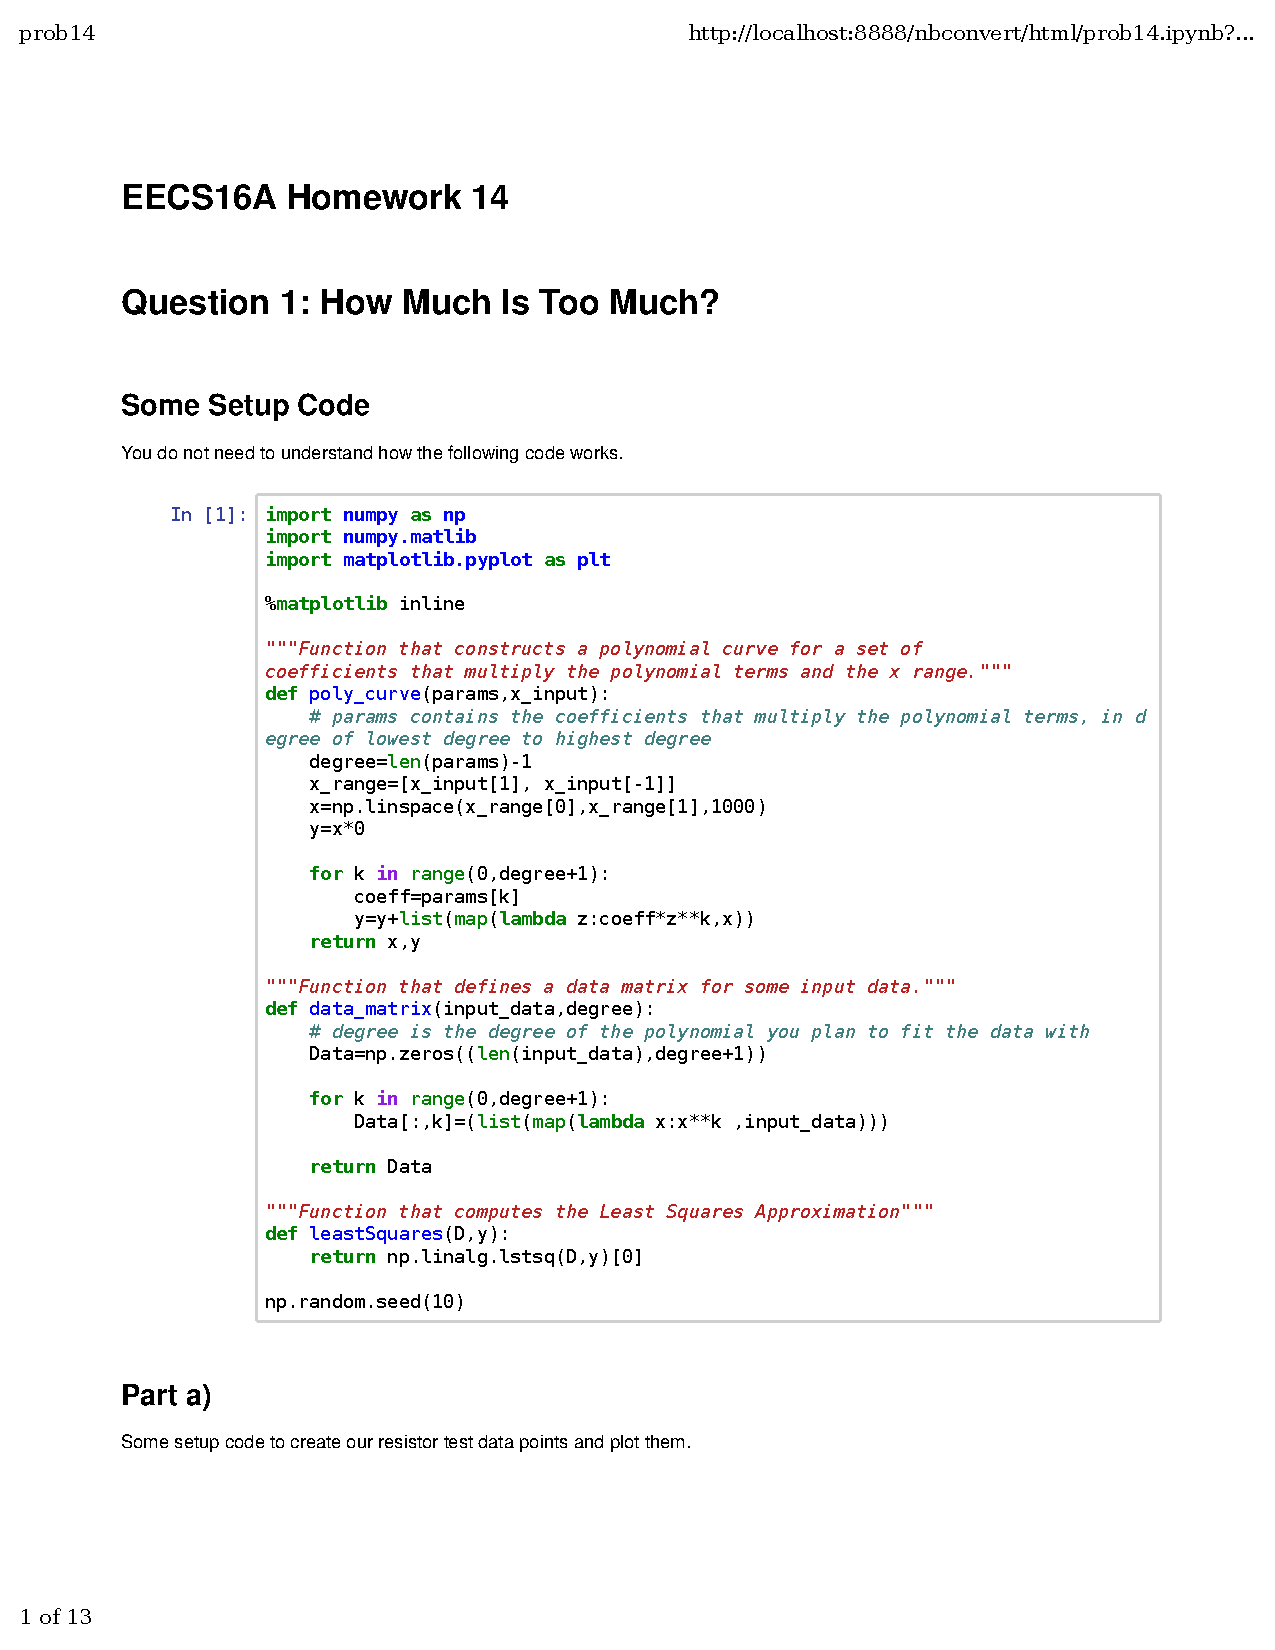
\includepdf[pages=-]{prob14.pdf}
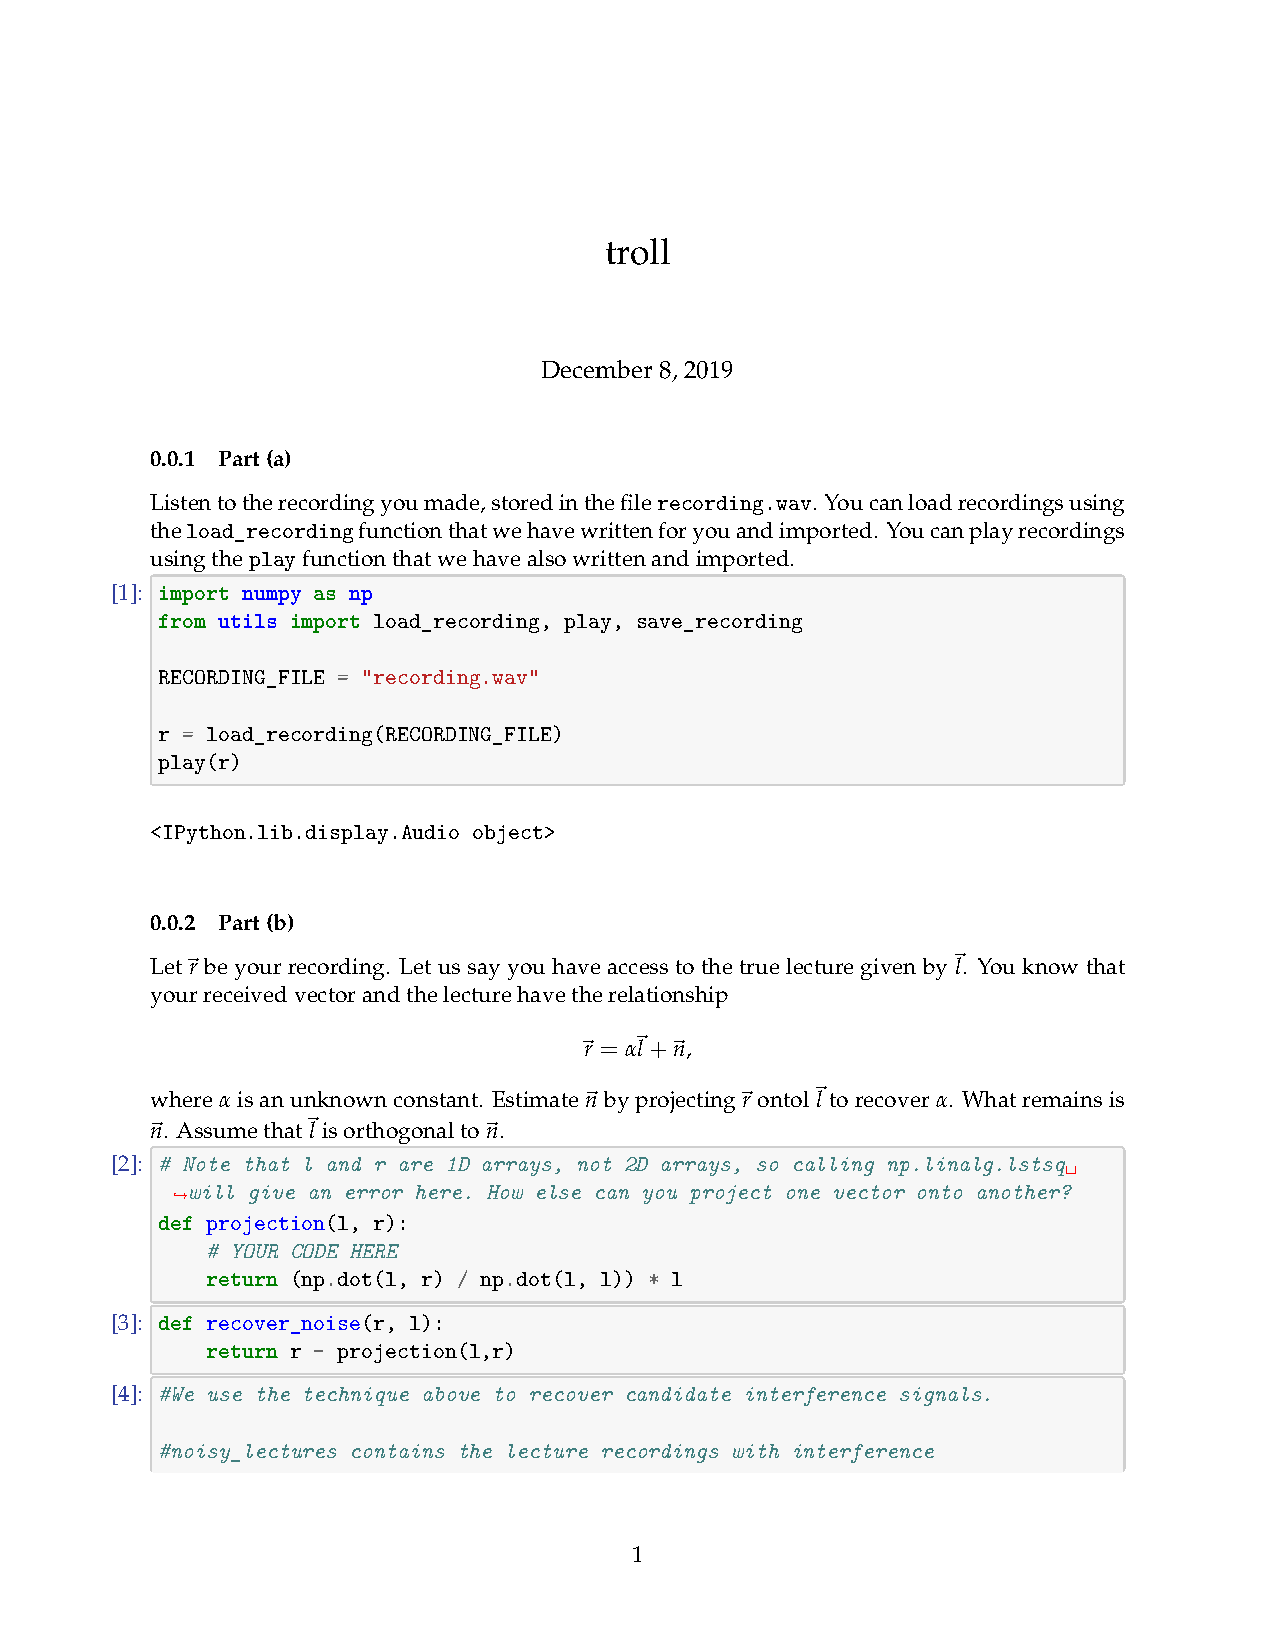
\includepdf[pages=-]{troll.pdf}

\end{document}
